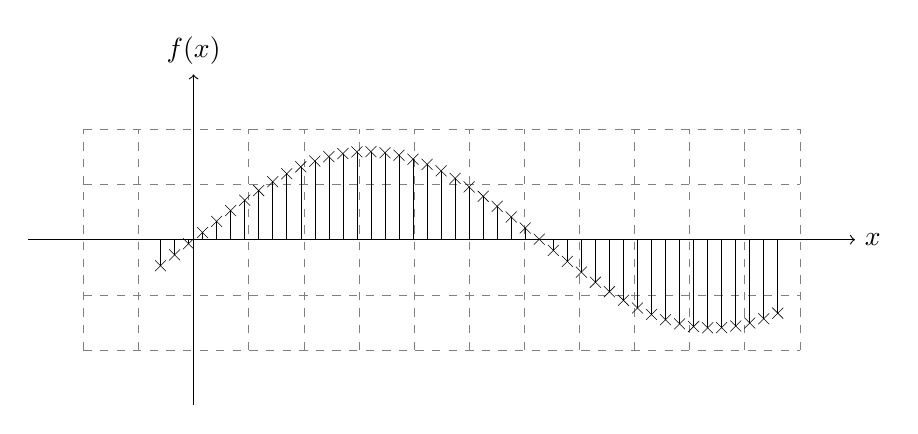
\begin{tikzpicture}[scale=1.4]
%grid
\draw[very thin,color=gray,step=.5cm,dashed] (-1,-1.0) grid (5.5,1);
\draw[->,color=black] (0,-1.5) -- (0,1.5)  node [above]{$f(x)$};
\draw[->,color=black] (-1.5,0) --  (6,0) node [right] {$x$};  
\draw[very thin,color=black,samples=45,domain=-0.3:5.3] 
plot[ycomb,thin,mark=x] (\x, { 0.8 * sin(\x r) });  
\end{tikzpicture}